\documentclass[paper=a4,11pt,bibliography=totoc]{scrartcl}
%\usepackage{fourier}

\usepackage[utf8]{inputenc}
\usepackage[english]{babel} 
%\usepackage[round,sort,authoryear]{natbib}
\usepackage{hyperref}
\usepackage{url}
\usepackage[protrusion=true,expansion=true]{microtype}
\usepackage{amsmath,amsfonts,amsthm, amssymb}
\usepackage[pdftex]{graphicx}
% \usepackage{subfigure}
\usepackage{longtable}
\usepackage{float}
\restylefloat{table}
\usepackage{tabularx}
%\usepackage{todonotes}
\usepackage{booktabs}
% \usepackage{framed}
\usepackage{listings}
%\usepackage{newclude}
\usepackage{enumerate}
\usepackage{color}
\usepackage{setspace}

\usepackage{mathtools}
\DeclarePairedDelimiter\ceil{\lceil}{\rceil}
\DeclarePairedDelimiter\floor{\lfloor}{\rfloor}



%\onehalfspacing
\parskip 3mm
% Verhindert die Einrückung der Absätze
\setlength{\parindent}{0pt}

% units and refs
\usepackage{xspace}
\usepackage{siunitx}
\usepackage{hyperref}
\usepackage[nameinlink]{cleveref}
\usepackage{appendix}

\usepackage{xcolor}
\hypersetup{
    colorlinks,
    linkcolor={red!50!black},
    citecolor={gray!80!black},
    urlcolor={gray!80!black}
}

\usepackage{epigraph}

%%%%%%%%%%%%% Options %%%%%%%%%%%%%
% \captionsetup{justification=centerlast} comment by Lukas
\sisetup{range-units=single}

%%%%%%%%%%%%% Ref maps %%%%%%%%%%%%%
\def\eq#1{\textcolor{red!50!black}{Eq.}~\labelcref{#1}}
% \renewcommand{\eq}{def}
%%%%%%%%%%%%%%%%%%%%%%%%%%%

%%%%%%%%%%%%% Graphic paths %%%%%%%%%%%%%
\graphicspath{{./figures/}}

\definecolor{greey}{RGB}{89, 89, 89}

\newcommand*{\fullref}[1]{\hyperref[{#1}]{\ref{#1} \nameref*{#1}}}

\newcommand\mw[1]{\textcolor{red}{#1}}

\setcounter{secnumdepth}{5}
\setcounter{tocdepth}{5}

\title{\vspace*{5cm}\onehalfspacing{Visualising the Functional Renormalisation Group}}
\subtitle{\vspace*{1.4cm}\onehalfspacing Universität Heidelberg\\-- Project report --\\Fortgeschrittenenpraktikum (2018/2019)\\[0.4in]
	%\onehalfspacing{In collaboration with Jan M. Pawlowski and Filip Sadlp}\\[0.4in]
}

\author{Lukas Kades}

\date{\today}


\begin{document}
\maketitle
\thispagestyle{empty}
\newpage
\setcounter{page}{1}
\renewcommand{\contentsname}{I Contents}
\renewcommand{\refname}{II References}
\addcontentsline{toc}{section}{I Contents}
\tableofcontents

\newpage 

\definecolor{darkgreen}{rgb}{0,0.39,0} 
\definecolor{darkred}{rgb}{0.39,0,0}
\definecolor{lightblue}{rgb}{0.063,0.14,0.59}

\epigraph{\textit{A theory is said to be asymptotically safe if the essential coupling parameters approach a fixed point as the momentum scale of their renormalisation point goes to infinity.}}{\textit{Steven Weinberg}~\cite{Weinberg1980}}

\section{Introduction}
\label{sec:intro}

We present a software framework which is capable of finding and characterising critical points of a set of coupled ordinary differential equations (ODEs). The algorithms are implemented in a parallel manner and can be executed on GPUs. Our work is motivated by a growing computational cost for the detection of fixed points for an increased number of differential equations. Such large sets of ODEs need to be solved within a certain approximation of the Wetterich equation based on the functional renormalisation group (FRG)~\cite{Pawlowski2018}. In this equation, the concept of renormalisation group of quantum and statistical field theory is implemented as the functional renormalisation group. The equation is heavily used within the field of research of quantum chromo dynamics (QCD) and quantum gravity, for example. The knowledge about critical points of a physical theory provides valuable insights into properties and characteristics of the underlying theory on different physical scales. It should also be mentioned that the software framework is not restricted to this particular use case but is implemented for more generic applications.

\subsection{Physical Motivation}

The Wetterich equation, which is also referred to as functional renormalisation group equation or flow equation, is the key equation of the FRG. In most cases, the flow equation, which is an exact equation, cannot be solved numerically. Therefore, the equation must be truncated in practice, i.e., approximated. This is achieved, for example, by a projection into a sub-theory space which is spanned by time-dependent variables, so called couplings or coupling constants. A set of ODEs is build up by these couplings whereas the number of couplings determines the dimension of the considered problem. The considered space is spanned by the couplings and is referred to as theory space. In this project, we concentrate on this kind of approximation to solve the Wetterich equation. A respective solution helps to understand macroscopic states of the system and allows to study the critical behaviour of the theory. This includes the computation of critical exponents and the identification with a certain universality class as well as a consideration of phase transitions and spontaneous symmetry breaking. Further, a characterisation of the fixed point with respect to the directions of incoming and outgoing flow enables a determination of the number of physical parameters which need to be fixed in the considered theory.

Numeric solutions of flow equations are limited for a growing number of ODEs by the high complexity of the equations itself and the resulting high dimension. However, the accuracy of obtained results and predictions dependents on the dimension of the considered sub-theory space. In general, it holds: The larger the number of ordinary differential equations, the more complex the respective flow equations and the more accurate are the solutions. This property represents together with the physical gain of solving the Wetterich equation the main motivation of this project. We expect that an extension to further approaches for solving the flow equation or at least to flow equations with a different inherent structure is in most cases easily to implement due to the modular structure of the software.

\subsection{Main Contributions - Properties of the Developed Software}

The developed software is optimised to gain a performance boost by parallising the computation of a generic coupled set of ordinary differential equations (ODEs). We aim at a computationally efficient, parallel evaluation of ODEs for many different initial arguments on a grid. Therefore, we do not focus on the integration of a very large set of differential equations within this project. A generic meta programming module written in Python enables a generation of Thrust code for ODEs of arbitrary complexity. The code is generated by parsing the ODEs from a \textit{.txt} file that includes the mathematical expressions. The main module of the project is written in C++/Thrust. It provides an interface to be able to access and to call the generated Thrust code for an evaluation of the ODEs on the GPU. The module contains implementations of different numeric methods to deduce properties of the ODEs. This includes a systematic search for roots of the ODEs, i.e., for fixed/critical points, a computation of the Jacobi matrix, and a possible numerical integration of the differential equations. The latter is utilised for the computation of separatrices. The set of differential equations can be interpreted as a description of a flow in higher dimensional space. This space is spanned by the flow of variables which is described by the set of ODEs~\cite{Asimov2003}. Therefore, the dimension is given by the number of ODEs. The results can be visualised in arbitrary pairs of dimensions. The development of more meaningful and effective visualisation methods, similar to~\cite{Noll1967} and~\cite{Hofmann2018}, is subject to future work.

The software is implemented with the goal of a modular structure. It should be easy to extend, modify, replace or detach certain components for a customised usage. Currently, the features of the software aim particularly at a convenient and efficient way to evaluate flow equations which emerge in computations within the functional renormalisation group. Nevertheless, the code can be easily adapted to an evaluation of an arbitrary set of differential equations.

\subsection{Related Work}

To the best of our knowledge, no suitable software exists for the detection of fixed points in arbitrary higher dimensional spaces with a respective implementation on a GPU. A four dimensional flow is studied, for example, in~\cite{Noll1967}. Methods for a visualisation of 4d vector field topology were introduced recently in~\cite{Hofmann2018}. In quantum gravity, theory spaces with very high dimensions are considered. The systems range from a few dimensions to systems with more than thirty dimensions. For recent work on the analysis of fixed points in quantum gravity and with respect to the asymptotic safety, see, for example,~\cite{Braun2010, Nicolai2018} or~\cite{Eichhorn2018, Eichhorn2019, Pawlowski2019}. The search for fixed points is performed mainly within the computer algebra program Mathematica due to the high dimension of the theory space and rather complex analytic ODEs of the flow. In QCD, certain frameworks exist for the generation, computation and evaluation of flow equations, see, for example~\cite{Cyrol2017,Huber2012,Mitter2015}. However, their features concentrate mainly on other expansion schemes or other formulations of the functional renormalisation group and are not suited for an efficient detection of fixed points in quantum gravity.

\subsection{Project Structure and Workflow}
\label{sec:proj}

This sections reveals the different stages and subtasks which have been run through during the project. It provides an insight into the workflow during the project as well as a deeper understanding of the developed software.

\textbf{Stage 1: Theoretical background}
\begin{center}
	\leftskip4em\small The basic concepts and applications of the functional renormalisation group are studied by attending lectures, self-study and discussions. The flow equations, as the key equation of the FRG, are formulated as a coupled set of ordinary differential equations. The resulting generic mathematical description serves as a starting point for a possible evaluation based on visual computing.
\end{center}

\textbf{Stage 2: Getting used to Thrust}
\begin{center}
	\leftskip4em\small The parallel algorithm library Thrust is installed successfully on the different used devices (Laptop, GPU Cluster, IWR Grahiklabor). The semantic as well as the features of the library are learned by running first basic examples.
\end{center}

\textbf{Stage 3: Development and implementation of a packaging/indexing method of vertices}
\begin{center}
	\leftskip4em\small A processing procedure is implemented to be able to evaluate the flow equations efficiently and highly parallelised on a grid. For optimisation purposes, data traffic between the CPU and the GPU is kept as small as possible. The grid consists of hypercubes. A recursive partition of a hypercube into smaller hypercubes is necessary for a latter computation of fixed points. An indexing method for these hypercubes is developed for a unique identification of each hypercube regardless of the depth of the recursion procedure.
\end{center}

\textbf{Stage 4: Preparation of the flow equation into a generic form}
\begin{center}
	\leftskip4em\small The flow equations usually result from analytic expressions in Mathematica. The equations are transferred into a generic data format to be able to work with those in Thrust. The data format is given by a tree like representation of the equations in a standard \textit{.txt} file format.
\end{center}

\textbf{Stage 5: Parsing the flow equations with Python}
\begin{center}
	\leftskip4em\small The generic flow equations are parsed with the help of Python as a preparation for Stage 6. Every string of the mathematical tree like structure is assigned a semantic meaning within this process. The tree is represented in Python by a so called pandas DataFrame as a result of this stage.
\end{center}

\textbf{Stage 6: Meta programming for the generation of Thrust code}
\begin{center}
	\leftskip4em\small The parsed flow equations enable an understanding of the underlying algebra and mathematical expressions of the flow equations. Thrust code is generated based on the tree of scoped algebraic computations. The Thrust code is executable on a GPU and is easily accessible by standard algorithms of Thrust.
\end{center}

\textbf{Stage 7: Detecting fixed points of the flow equations}
\begin{center}
	\leftskip4em\small Within the previous stages, all necessary components have been developed for an efficient evaluation of the flow equations and, respectively, of a generic coupled set of ordinary differential equations based on Thrust. The components are combined in an interface that allows the detection of fixed points based on a recursive partition of hypercubes. The partition is governed by a certain criterion that allows the detection of potential fixed points within a hypercube.
\end{center}

\textbf{Stage 8: Extension of the C++ code by further useful methods (stability matrix, 
critical exponents, integration with boost)}
\begin{center}
	\leftskip4em\small Further functionalities are implemented for a proper investigation of the found fixed points. This includes a computation of the stability matrix and the critical exponents. Further, a numerical integration method is provided that allows, for example, the extraction of separatrices. This can be understood as the study of some flow which starts in the vicinity of a fixed point.
\end{center}


A more detailed description of the different stages is given in the next sections with an emphasis on theoretical aspects of the used methods and techniques. Work on the stages was partially mixed during the project. The report is structured as follows. \Cref{sec:physicsfunamentals} provides an introduction to the functional renormalisation group and derives a description of a possible implementation in terms of a set of ordinary differential equations. We proceed in~\Cref{sec:vft} with a repetition of important methods in vector field topology. The section highlights links between these methods and procedures for the description of characteristics of a physical theory. In~\Cref{sec:algorithms}, the most important developed algorithms are presented in detail, with an emphasis on an efficient implementation of a fixed point search algorithm on the CPU and GPU. The performance of the software framework is evaluated with respect to a comparison between CPU and GPU run times in~\Cref{sec:performance}. The conclusion and an outlook can be found in~\Cref{sec:conc}.

\section{Physics Fundamentals}
\label{sec:physicsfunamentals}
%
The section introduces the idea of the functional renormalisation group in theoretical physics. The Wetterich equation is discussed and a set of ordinary differential equations is derived starting from the example of scalar theory. The interest in physics is motivated by a reasonable detection and interpretation of critical points of the underlying theory based on a solution of the given set of ODEs. The section follows partly the lecture notes in~\cite{Pawlowski2018}.
%
\subsection{The Renormalisation Group}
\label{sec:ren}
%
The renormalisation group (RG) describes the change of physical quantities with respect to different length scales. It can be understood as the investigation of a high-resolution image which is subsequently coarse grained. In terms of physics this corresponds to a smooth interpolation between microscopic physical laws and macroscopic collective phenomena. In other words, microscopic details are averaged out when going to higher resolutions. The functional renormalisation group (FRG) describes such a coarse graining in moment space. It can be interpreted as a continuous version of the Kadanoff block spinning idea~\cite{Kadanoff} which was introduced on the lattice by Wilson in~\cite{Wilson1971, Wilson1971b}. The concept is used in quantum and statistical field theories, especially for the investigation of system which are only non-perturbatively accessible, as, for example, strongly correlated systems and quantum gravity. In FRG, the RG flow takes place in theory space. This space is spanned by all couplings that define the considered theory.

Studying the flow enables the detection of critical points. These correspond to points where a change in scale, i.e., a renormalisation group step, does not change the physics of the system. Accordingly, the theory becomes scale independent~\cite{Pawlowski2018, WikiFrg}. One motivation to find such fixed points originates from the concept of asymptotic safety in quantum gravity. It aims to find a consistent and predictive quantum theory of the gravitational field. In other words, this corresponds to a RG trajectory in theory space which is well-behaved for arbitrary momentum scales. The idea is to find a quantum field theory that allows a smooth transition from low energies to a more general quantum field theory which is also well-defined for energies above a certain threshold value of the momentum or energy scale, respectively. This is known as UV completion and enables the detection of theories with physical quantities that are safe from divergences in the ultraviolet (UV) regime for high energies~\cite{WikiAsym}. A Gaussian fixed point describes a free theory with vanishing couplings. These theories are perturbatively accessible. The existence of non-trivial (non-Gaussian) fixed points allows to generalise the procedure of perturbative renormalisation in the sense that all couplings can be finite and do not diverge. The concept of asymptotic freedom is discussed again in~\Cref{sec:anaf} when critical points are characterised.
%

\subsection{The Wetterich Equation}
\label{sec:wett}

The basic flow equation which describes the renormalisation group flow is given by the Wetterich equation~\cite{Wetterich1993}, which is also referred to as the functional renormalisation group equation
%
\begin{equation}
\label{eq:wetterich}
\partial_t \Gamma_k[\phi]=\frac12\textnormal{Tr}\frac{1}{\Gamma_k^{(2)}[\phi]+R_k} \partial_t R_k=\frac12 \int\displaylimits_p\frac{1}{\Gamma_k^{(2)}[\phi]+R_k(p^2)}(p, -p)\partial_t R_k(p^2)\,,
\end{equation}
%
where $\int\displaylimits_p = \int \frac{\textnormal{d}^dp}{(2\pi)^d}$. The flow equation is explained in the following step by step. $\Gamma_k[\phi]$ corresponds to the scale-dependent or flowing effective action. The term \textit{scale-dependent} refers to the index $k$, which is defined by the RG time $t=:\ln k/\Lambda$. The index indicates that the flowing effective action contains all quantum and statistical fluctuations with momenta $q \gtrsim k$~\cite{WikiFrg}. The upper index $(n)$ of the flowing effective action $\Gamma_k[\phi]$ indicates the $n$-th functional derivative with respect to $\phi$, i.e.,
%
\begin{equation}
\Gamma_k^{(n)}[x_1,\ldots,x_n] := \frac{\delta^n \Gamma_k}{\delta\phi(x_1)\ldots\delta\phi(x_n)}\,.
\end{equation}

The effective action $\Gamma[\phi]$ is the generating functional of 1PI correlation functions for some mean field $\phi(x) = \langle\varphi(x)\rangle$. The generating functional contains all relevant information of the considered physical system. This includes the considered theory and the respective physical parameters. Accordingly, if the effective action is known, it is possible to compute n-point correlation functions $\langle \varphi(x_1)\cdots \varphi(x_n)\rangle$ as observables of physical interest.

The RG time $t$ is the time which the flow takes place in. The cutoff scale $\Lambda$ is a fixed physical, intrinsic, reference scale and determines where the flow is initiated. It corresponds to the scale where all quantum fluctuations are suppressed. Having our coarse grained picture in mind, the physical system is well-described by the microscopic quantities of the system. Our physical system is perturbatively accessible at this scale. In QCD, this is the scale below which strong correlations take place~\cite{Pawlowski2018}. The direction of the flow depends on the considered physical theory. As described in the previous section, one is interested in the behaviour of the theory in the UV limit. This corresponds to a flow to high energy scales and to the limit $k\to\infty$. In general, it holds that the length scale which can be resolved is the lower the higher the energy or momentum scale. In contrast, in QCD, the idea is to start from a classical action at the physical reference scale $k=\Lambda$ to arrive at the full quantum effective action at $k=0$. Accordingly, the flow runs from $t=0$ to $t\to-\infty$ if we consider a flow starting from $k=\Lambda$ and ending at $k=0$. Each infinitesimal RG step incorporates more and more quantum fluctuations into the effective average action. At $k=0$, all quantum fluctuations are integrated out with the help of the flow equation. The latter limit is also denoted as infrared (IR) limit since this refers to lower energy and momentum scales. The functional renormalisation flow enables a solution of the theory in an iterative manner, momentum shell for momentum shell. In concordance with the apparatus of renormalisation group, it interpolates between a bare action $\Gamma_{k=\lambda}[\phi]$ and the full quantum effective action $\Gamma_{k=0}[\phi]$. The scale derivative $\partial_t R_k(p^2)$ of the regulator function $R_k(p^2)$ is the technical feature which makes this possible. It has a peak around $k$. The regulator function itself converges to $k^2$ for $p^2 \ll k^2$ and vanishes for $p^2 \gg k^2$. It can be interpreted as a dynamical mass that suppresses the propagation of momentum modes for momenta $p^2\lesssim k^2$ and has no impact on the propagation of momenta $p^2 \gtrsim k^2$. In the limit of $k=0$ the cutoff term vanishes and the solution is independent of the chosen infrared regularisation procedure. \Cref{fig:uvir} depicts this procedure and indicates with the different trajectories a freedom of the choice of the regulator function~\cite{Pawlowski2018}.

\begin{figure*}
	\centering\includegraphics[width=0.46\textwidth]{Theoryspace.png}
	\caption{Depiction of the flow of the functional renormalisation group in theory space which is spanned by the different coupling constants of the theory. The Wetterich equation~\eq{eq:wetterich} enables an interpolation between the bare action $\Gamma_{k=\Lambda}[\phi]$ and the full quantum effective action $\Gamma_{k=0}$. The different trajectories indicate that the start and end point does not depend on the chosen regulator function $R_k(p^2)$. Nevertheless, the regulator function needs to fulfill certain characteristics, for details, see~\cite{Pawlowski2018}. (Scheme taken from~\cite{WikiRen})}
	\label{fig:uvir}
\end{figure*}

Expressed in formulas, an integration of the flow equation can be understood as a solution of the full effective action in the sense that
%
\begin{equation}
\label{eq:integratedflow}
\Gamma[\phi] = \int\displaylimits_\Lambda^0 \frac{dk}{k} \partial_t \Gamma_k[\phi] + \Gamma_\Lambda[\phi]\,,
\end{equation}
%
where $\Gamma_\Lambda[\phi]$ can be expressed in terms of the field $\phi$ and additional physical parameters, which are given for the scaler theory by
\begin{equation}
\Gamma_\Lambda[\phi]= \Gamma_\Lambda\left[\phi; Z_{\phi, \Lambda}, m_\Lambda^2,\lambda_\Lambda\right]\,.
\end{equation}
%
Here, $Z_{\phi, \Lambda}$, $m_\Lambda^2$ and $\lambda_\Lambda$ correspond to fixed values for the couplings of the $\varphi^4$-theory at $k=\lambda$, which is an example of an interesting physical system. Initial conditions are implemented into the flow equation based on the above equation~\eq{eq:integratedflow} under the heuristic expectation that in the ultraviolet limit the effective action convergence towards the classical one, i.e.,
%
\begin{equation}
\lim\limits_{k\to\infty}\Gamma_\Lambda[\phi] = S_\textnormal{UV}[\phi, R_\Lambda]\,,
\end{equation}
%
where the theory is perturbatively accessible.

\subsection{$\varphi^4$-Theory}

In the next section, a possible approach to solve the Wetterich equation by an approximation is introduced based on the example of the $\varphi^4$ scalar theory. Therefore we briefly introduce this theory which corresponds to a quantum field theory that is often used for illustrative and introductory purposes.

The classical action of the theory is given by:
%
\begin{equation}
\label{eq:scalartheory}
S[\varphi]=\int\displaylimits_x \left[\frac12 Z_\varphi \partial_\mu \varphi(x)\partial_\mu \varphi(x) + \frac{m^2}{2}\varphi(x)^2 + \frac{\lambda}{4!}\varphi(x)^4\right]\,,
\end{equation}
%
with $\int\displaylimits_x = \int \textnormal{d}^dx$. A scalar field describes a spin-zero particle in space time. Within the action, $m$ can be identified with the mass of the particle and $\lambda$ corresponds to the interacting coupling and determines the strength of the interaction between particles. The wave function renormalisation $Z_\varphi$ takes care of higher order loop corrections. The action is composed of a kinetic term, given by the first term, and a potential $V(\varphi)$ consisting of a mass term and an interaction term with coupling $\lambda$. The field is defined by a mapping of the four dimensional space time vector $x^\mu = (t, \vec{x})$ onto a scalar field
%
\begin{equation}
\varphi: x^\mu \rightarrow \varphi(x^\mu)\equiv \varphi(x) \in \mathbb{R}\,.
\end{equation}
%
The partial derivative is given by
%
\begin{equation}
\partial_\mu \varphi(x) = \frac{\partial}{\partial x^\mu} \varphi(x)\,.
\end{equation}

\subsection{Solving the Wetterich Equation}

With the above given framework at hand, a possible approach for solving the Wetterich equation is presented in the following on the basis of the scalar theory. We choose \textit{derivative expansion} as one of the possible systematic expansion schemes for solving the flow equation. The idea of the derivative expansion is to systematically add derivatives of higher orders of the quantum corrections of the theory. This expansion scheme makes use of a possible expansion of the effective theory at low energies. For further details see~\cite{Pawlowski2018}.

The flowing effective action can be defined in this approximation, which is also referred to as \textit{Local Potential Approximation} (LPA), by
%
\begin{equation}
\label{eq:lpa}
\Gamma_k[\phi]=\int\displaylimits_x \left(\frac{1}{2}\partial_\mu \phi \partial_\mu \phi + V_k(\rho) + \mathcal{O}\left(\partial^2\right)\right)\,,
\end{equation}
%
where $\rho:=\frac{\phi^2}{2}$ is introduced for convenience. The order $\mathcal{O}\left(\partial^2\right)$ applies only to quantum fluctuations, i.e., does not affect the classical kinetic term. \eq{eq:lpa} serves as an ansatz for the flowing effective action. The \textit{effective potential} $V_k(\rho)$ can, in principle, contain terms of arbitrary order in $\rho$. However, terms of odd order in $\phi$ are not presented due to a $Z_2$-symmetry of the scaler field theory under $\phi\to-\phi$.

For our example of the scaler theory~\eq{eq:scalartheory}, the effective potential is given in the classical limit by
%
\begin{equation}
V_\Lambda(\rho)=m_\Lambda^2 \rho + \frac{\lambda_\Lambda}{3!}\rho^2\,,
\end{equation}
%
where the dependence of the initial conditions on $m_\lambda^2$ and $\lambda_\Lambda$ can be immediately seen.

A possible solution of the flow equation is parametrised by a polynomial expansion of the effective potential in $\rho$
%
\begin{equation}
\label{eq:polyexpansion}
V(\rho)=\sum_{n=0}^\infty \frac{\lambda_n}{n!}\left(\rho-\kappa\right)^n\,.
\end{equation}
%

The expansion point $\kappa$ is often chosen to be the cutoff-dependent minimum of the effective potential $\phi_{0, k}$, which is defined by
%
\begin{equation}
\frac{\partial V_k(\rho)}{\partial \phi}\bigg|_{\phi=\phi_{0, k}}=0\,.
\end{equation}
%
The latter equality comprises an algebraic constraint on the solution of the flow equation. In this case a further flow equation needs to be derived for $\kappa$. In the further considerations, we restrict ourselves to a solution of the flow equation for a fixed expansion point $\kappa$.

The ansatz of~\eq{eq:lpa} is inserted together with a polynomial expansion of the flowing, i.e., scale dependent, effective potential $V_k(\rho)$ into the Wetterich equation~\eq{eq:wetterich}. Following the computations in~\cite{Pawlowski2018}, one arrives at the following flow equation:
%
\begin{equation}
\partial_t V_k(\rho) = \frac{\Omega_d}{(2\pi)^d}\frac{k^{d+2}}{d}\frac{1}{k^2+V_k'(\rho)+2\rho V_k''(\rho)}\,.
\end{equation}
%
Based on the LPA ansatz, the flow of the flowing effective action $\Gamma_k[\phi]$ has been transformed into a flow of the flowing effective potential $V_k(\rho)$. This can be rewritten into a generic expression of the following form:
%
\begin{equation}
\partial_t V_k(\rho) = F_k\left(\rho, V_k'(\rho), V_k''(\rho)\right)\,.
\end{equation}
%
For other physical systems, such an expression can also be derived.

The $\lambda_n$ represent the only left quantities of the polynomial expansion with a possible $k$-dependence. Flow equations for these scalar functions can be obtained by derivatives of the flow equation with respect to $\rho$ and by evaluating the resulting equations at the expansion point $\kappa$. This leads with
%
\begin{equation}
\frac{\partial^j}{\partial \rho^j} V(\rho)\bigg|_{\rho=\kappa} = \frac{\partial^j}{\partial \rho^j} \sum_{n=0}^\infty \frac{\lambda_n}{n!}\left(\rho-\kappa\right)^n\bigg|_{\rho=\kappa} = \lambda_j(k)
\end{equation}
%
and
%
\begin{equation}
f_j(k, \lambda_1(k), \ldots, \lambda_{j+2}(k)):= \frac{\partial^j}{\partial \rho^j} F_k\left(\rho, V_k'(\rho), V_k''(\rho)\right)\bigg|_{\rho=\kappa}
\end{equation}
%
to the following set of ordinary differential equations
%
\begin{align}
\partial_t \lambda_0(k) &= f_0(k, \lambda_1(k), \lambda_2(k))\,,\nonumber\\[1ex]
\partial_t \lambda_1(k) &= f_1(k, \lambda_1(k), \lambda_2(k), \lambda_3(k))\,,\nonumber\\[1ex]
&\colon\nonumber\\[1ex]
\partial_t \lambda_j(k) &= f_j(k, \lambda_1(k), \ldots, \lambda_{j+2}(k))\,,\nonumber\\[1ex]
&\colon
\end{align}
%
where we have used that $\frac{\partial}{\partial t}=\frac{\partial k}{\partial t}\frac{\partial}{\partial k}=k \frac{\partial}{\partial k}$.

We truncate the polynomial expansion at order $n$ for a numerical computation. Based on this truncation, the theory is projected on some finite-dimensional sub-theory space. Introducing the vector $\vec{\lambda}=\left(\lambda_0(k), \lambda_1(k), \ldots, \lambda_n(k)\right)$, the system of ordinary differential equations can be rewritten as a vector flow equation:
%
\begin{equation}
\label{eq:vecflowequation}
\partial_t \vec{\lambda}(k) = \vec{f}(k, \vec{\lambda}(k))\,.
\end{equation}
%
Initial conditions are given with respect to the initial potential according to:
%
\begin{equation}
\lambda_j(k=\Lambda) = \frac{\partial^j}{\partial \rho^j} V_\Lambda(\rho)\bigg|_{\rho=\kappa}\,.
\end{equation}

Keeping in mind the derivation of these equations based on the LPA ansatz, it is obvious, that the different couplings $\lambda_j$ span our theory space. The RG flow of our flowing effective action turned into a flow of the couplings of the flowing effective action. A solution of the flow equation for a particular initial condition corresponds in this space to a single trajectory with respect to the considered momentum scale. A vector field can be generated by solving the flow equation for a set of different initial conditions. With respect to the introduction of the renormalisation group in~\Cref{sec:ren} and of the Wetterich equation in~\Cref{sec:wett}, the idea of the functional renormalisation group should be more clear, now. The scale dependence of the flowing effective action is encoded in the change of the couplings. The couplings are also denoted as \textit{running couplings}. The RG flow helps to investigate macroscopic and microscopic quantities of the theory at different scales.

Written in this form, the couplings $\lambda_{j}$ carry a momentum dimension which implies a rescaling of the coupling under a total rescaling. To get rid of this dependency, they are rescaled into dimensionless, scale invariant couplings $\hat{\lambda}_j$. The correct rescaling is derived by a consideration of the dimension of the different terms and couplings of the theory. We skip this derivation and refer the reader to~\cite{Pawlowski2018} for a detailed computation. The resulting flow equation for the dimensionless couplings is known as $\beta$-function:
%
\begin{equation}
\label{eq:betafunction}
\beta_{\lambda_j} = \partial_t\hat{\lambda}_j\,=\hat{f}_i\left({\vec{\hat{\lambda}}}\right).
\end{equation}
%
It serves as a starting point for the analysis of critical behaviour by the detection of fixed points of this equation. Due to their properties, fixed points correspond to configurations $\Gamma_k[\phi]$ which become independent of the scale $k$. They enable a computation of critical exponents, a possible identification of the theory with a universality class and the analysis of phase transitions. The mathematical expressions in the following sections are based on the dimensionful flow equations~\eq{eq:vecflowequation} and can, in principle, directly be applied on the $\beta$-function.

\section{Methods - Vector Field Topology}
\label{sec:vft}

A parallelised evaluation of a rather complex set of ODEs represents the main focus of this project, as has been pointed out already in the introduction in~\Cref{sec:intro}. The section provides insights into the used numerical methods to evaluate important characteristics and properties of the flow for a given set of equations. The section starts with clear definition of the used terminology. Afterwards, the utilised method for the detection of fixed points of the flow is described in detail. The section ends with a detailed investigation of the characteristics of the detected fixed points and a possible way to extract separatrices.

\subsection{Terminology}

The analysis of the \textit{flow equations} takes place in a higher-dimensional \textit{theory space} that is spanned by the different coupling constants of the set of ODEs. Therefore, the dimensionality $n$ corresponds to the number of given ordinary differential equations. With respect to the FRG, the different axes are labeled by the coupling constants. The detection of the fixed points demands a consideration of n-dimensional cubes within this space. The hypercube consists of \textit{vertices} that are connected by the \textit{edges} of the cube. A predefined set of hypercubes is referred to as \textit{collection}. A \textit{point} in the higher-dimensional theory space is defined by respective components in each dimension. \textit{Boundaries} of the considered theory space need to be defined a priori for the detection of fixed points since the applied numerical method requires a necessary minimum resolution of the entire space.

\subsection{Detection of Fixed Points}
\label{sec:DetectionOfFixedPoints}

We detect fixed points by the following recursive numerical method. The flow, i.e., the right hand side of the flow equation~\eq{eq:vecflowequation} or of the beta function~\eq{eq:betafunction} vanishes at a \textit{fixed point} or \textit{critical point} $\vec{\lambda}^\star$:
%
\begin{equation}
\partial_t \vec{\lambda}(k)\bigg|_{\vec{\lambda}^\star}=0\,.
\end{equation}
%
In a first step, the theory space is partitioned into a fixed number of hypercubes. The resolution of the resulting grid of hypercubes needs to be chosen based on experience and with respect to the predefined boundaries. In the next step, the flow equation is evaluated at each vertex of the given set of hypercubes. A potential fixed point within a given hypercube is detected in dependence on the sign of the resulting flow $\vec{f}$ by the following condition:

\begin{equation}
\label{eq:fixedpointdetection}
0 < \sum_{h=1}^{2^D} \Theta\left[f_d(k;\,h)\right] < 2^D\,,\quad\,\forall\, d\in\lbrace1,\ldots,D\rbrace\,,
\end{equation}

where $\Theta$ corresponds to the Heaviside function and the index $d$ to the component in dimension $d$. $D$ denotes the total dimension of the theory space. The sum runs over all vertices $h\in\lbrace 1, \ldots, 2^D\rbrace$ of the considered hypercube. The condition is satisfied if a change of the direction of the flow at the vertices of the hypercube takes place separately within each dimension.

If this condition is fulfilled, the hypercube is recursively partitioned into a new set hypercubes. Otherwise, the hypercube is dropped and not considered anymore. This recursive procedure results in the long run in a higher resolution of the fixed point in theory space. The only limiting factor is given by the numerical precision of the used device.

As pointed out, the condition~\eq{eq:fixedpointdetection} can be also fulfilled for hypercubes which contain no fixed point. An example is given together with a hypercube with an actual fixed point in~\Cref{fig:critpoints}. Most of these hypercubes with no actual fixed will be dropped within further recursion depth due to a finer resolution of the flow. Nevertheless, the condition will hold true in particular in vicinity of several critical points, for example, with rotational behaviour or for saddle points.

\begin{figure*}
	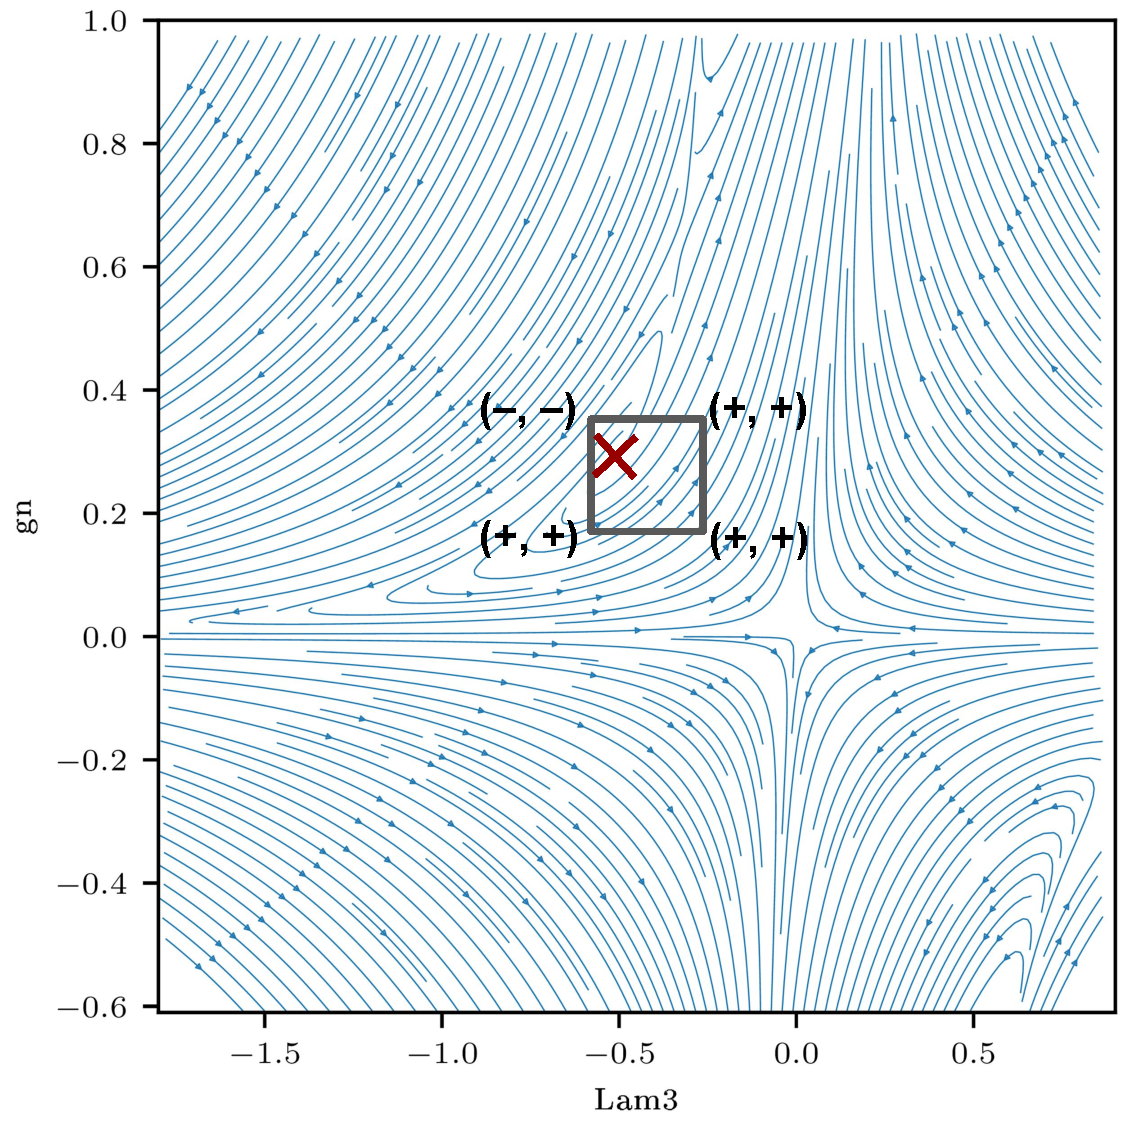
\includegraphics[width=0.48\textwidth]{FixedPoint}
	\hfill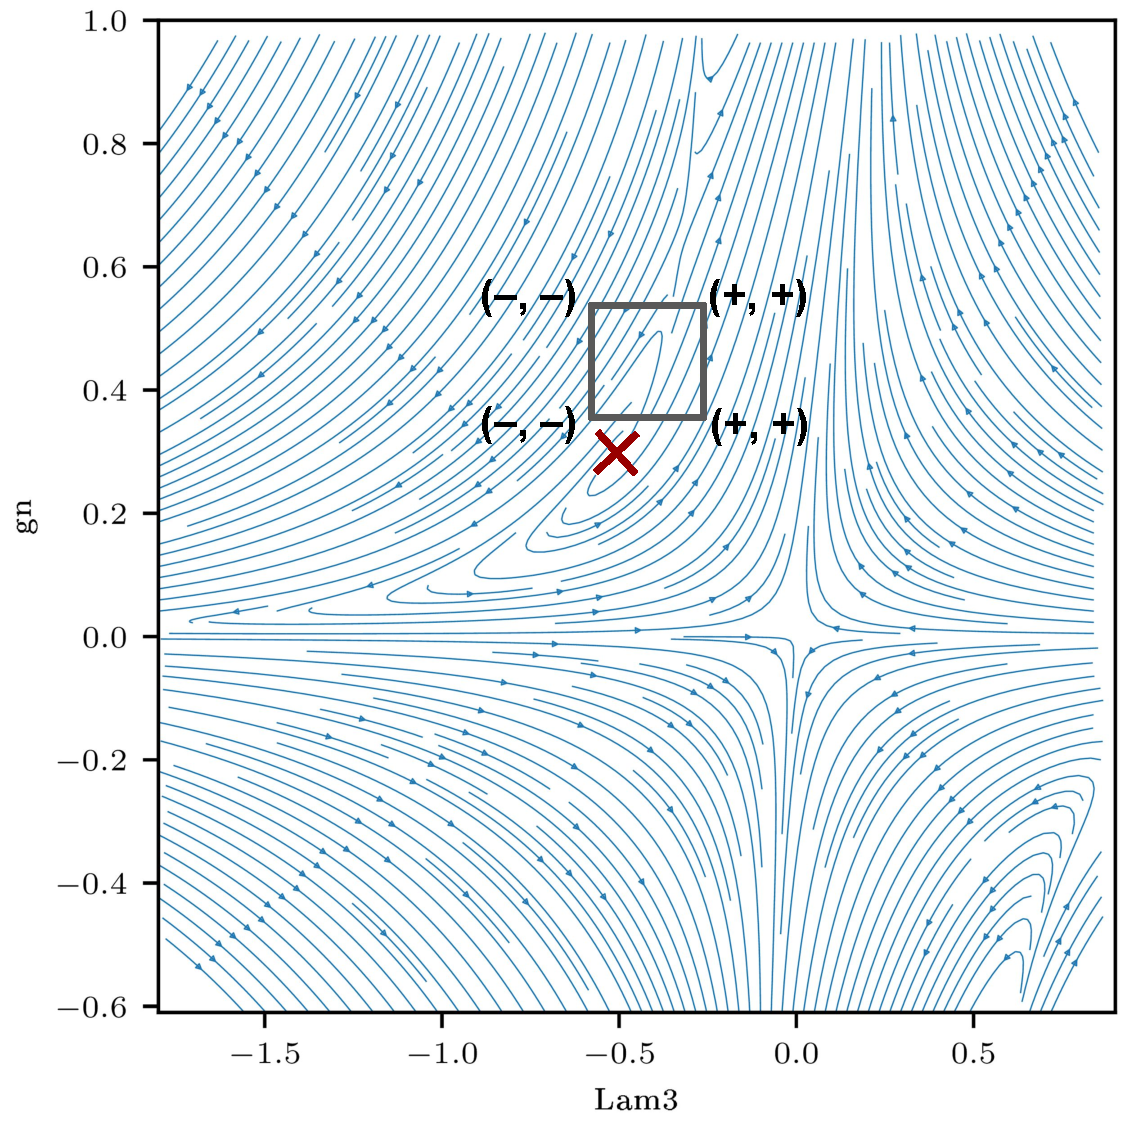
\includegraphics[width=0.48\textwidth]{PotentialFixedPoint}
	%\includegraphics[width=1.0\textwidth]{./figures/recon_distributionAllBW}
	\caption{Examples for the detection of potential fixed points based on the criterion~\eq{eq:fixedpointdetection}. The criterion holds if a change of the sign of the flow is detected in each dimension with respect to all vertices of the hypercube. The condition is fulfilled in both cases whereas only in the left illustration an actual fixed point is present within the hypercube.}
	\label{fig:critpoints}
\end{figure*}

The applied method for the detection of fixed points suffers under the following weaknesses. The predefined boundaries restrict a detection of fixed points outside of the resulting ranges. Further, the resolution of the hypercube has a decisive impact on the detection of fixed points. It is possible that nearby fixed points cancel the flow characteristic of fixed points in a wider region around them. Having a too coarse resolution, corresponding fixed points can not be detected. A possible approach to circumvent the latter weakness is the transition from a regular grid of hypercubes to an adaptive one. The resolution is determined based on characteristics and properties of the flow at the vertices of nearby hypercubes.

\subsection{Analysing Fixed Points}
\label{sec:anaf}

Having detected fixed points within the flow, it is interesting to study their properties. The stability of a fixed point is characterised by the interplay of the flow within the different dimensions. One common approach to analyse a fixed point is the investigation of the \textit{Jacobian matrix} $J$. The motivation to consider this matrix originates from a Taylor expansion around the fixed point $\vec{\lambda}^\star$ in the following manner:
%
\begin{align}
\partial_t \vec{\lambda}(k) &= \vec{f}(k, \vec{\lambda}(k))\bigg|_{\vec{\lambda}^\star} + \nabla\vec{f}(k, \vec{\lambda}(k)\bigg|_{\vec{\lambda}^\star} \left(\vec{\lambda} - \vec{\lambda}^\star\right) + \mathcal{O}\left(\left(\vec{\lambda} - \vec{\lambda}^\star\right)^2\right)\approx\nonumber\\ &\approx J \left(\vec{\lambda} - \vec{\lambda}^\star\right)\,.
\end{align}
%
The first term vanishes due to the properties of the fixed point itself to have a vanishing flow. Therefore the Jacobian matrix enables an analysis of the flow properties in the vicinity of the fixed point to first order. In this sense, it serves as a possibility to study the propagation of the flow  starting from a small change with respect to the fixed point. Within the FRG community, the Jacobian matrix is denotes as \textit{stability matrix}. The inverse of the eigenvalues of the stability matrix are the \textit{critical exponents} of the considered theory in the case of the $\beta$-function as corresponding flow equation. The critical exponents represent characteristics of the underlying system. It has been found that these exponents coincide for quite different physical systems. Theories with the same critical exponents are grouped in so called \textit{universality classes}~\cite{Wilson1974}. It turns out that theories of the same university class share the same relevant observables, i.e., they exhibit similar macroscopic physics despite different microscopic properties of the system~\cite{Scherer2018, Pawlowski2018}. The RG provides an explanation for the observed existence of universality which is build upon a more detailed analysis of the eigenvalue and eigenvectors.

The eigenvalues itself determine the structure of the flow around the fixed point. They are either real od complex conjugate pairs. The sign of a real part of the eigenvalue determines whether the flow into the direction of the associated eigenvector is attracting (positive real part) or repelling (negative real part). The given fixed point is a source if all eigenvalues are real and positive and a sink for sole real negative eigenvalues. A fixed point is \textit{structurally stable} if the real part of the eigenvalue is non-zero~\cite{Sadlo2017}. Rotational behaviour of the flow occurs for eigenvectors with non-negative imaginary part. In addition, a fixed point with at least one positive and at least one negative real part is called saddle. In particular in higher dimensions many different kinds of different flow structures can occur. Structures in three dimensions are, for example, a 1:2 \textit{saddle} with two real positive and one real negative eigenvalue or a 2:1 \textit{spiral source} with one real positive and two conjugate complex eigenvalues with negative real parts. In this notation, the first number defines the dimension of the incoming invariant manifold and the second one the dimension of the outgoing~\cite{Sadlo2017}.

The RG introduces a similar naming convention, motivated by the physical background. In quantum gravity one searches for theories that are safe from divergences in the UV limit, i.e., for momentum scales $k\to\infty$, for more details, see~\Cref{sec:ren}. A consistent and predictive quantum theory has been found if all coupling constants stay finite in the UV limit. With respect to this limit, the direction of an eigenvector with a negative real eigenvalue is called UV attractive or relevant since the flow hits the fixed point for $k\to\infty$. If one lowers the energy scale, the opposite holds. For this reason, the direction is also referred to as IR repulsive. In the same manner, a direction with a positive real eigenvalue is UV repulsive and IR attractive. In quantum gravity this corresponds to an irrelevant direction. Directions with a real eigenvalue equal to zero are called marginally relevant. Higher orders of the expansion around the critical point are necessary in order to determine the behaviour in the vicinity of the fixed point.  All relevant directions form the so called \textit{UV critical surface} for a saddle point. This surface corresponds to the invariant manifold where the couplings are pulled into a fixed point when flowing to larger energy scales. Accordingly, the statement of Steven Weinberg at the beginning of this report,~\Cref{sec:intro}, states that only these theories are asymptotically safe which are contained in the UV critical surface. Only these can occur in nature. Theories outside the surface diverge for $k\to\infty$~\cite{WikiAsym}. As a result, fixed points determine all possible macroscopic states of the system at a large momentum scale. Further, the number of relevant directions determines the number of physical parameters that need to be fixed~\cite{Scherer2018}. Once these relevant couplings are measured, the UV critical surface fixes the remaining irrelevant directions for arbitrary energy scales. This enables a fixing of, in principle, infinitely many couplings by a few relevant ones and renders the theory to a consistent and predictive quantum theory~\cite{WikiAsym}.

\subsection{Extracting Separatrices}

In dependence of the concrete application, it can be interesting to study so called \textit{separatrices}. These separate different modes of behaviour of the flow~\cite{Sadlo2017}. Separatrices can be mapped out by considering the propagation of the flow starting from the saddle points of the considered flow equations. The separatrix can be found by an integration of the flow equation. In other words, this corresponds to a streamline integration on a stable and an unstable invariant manifold starting from a saddle point. In general, a saddle point is characterised by attractive (belonging to the stable invariant manifold) and repelling (belonging to the unstable invariant manifold) directions of the flow which form these manifolds, respectively. The starting points are given by an infinitesimal, but finite, shift from the critical point into the direction of the respective eigenvector of the Jacobian matrix. The integration corresponds to a propagation of the starting points based on the streamlines of the flow. In dimensions larger than two, separatrices form higher-dimensional objects like hyperplanes and hypervolumes. The stable invariant manifold is build up by all eigenvectors with positive real part. Each eigenvector of eigenvalues with vanishing imaginary part correspond to a basis vector. The two basis vectors for complex conjugate pairs of eigenvectors are given by a first vector consisting of the real parts and a second vector which contains only the imaginary parts. The same holds for unstable invariant manifolds which is build by eigenvectors with negative real part. A complete representation and a suitable parametrisation get more complicated as a consequence of the more complex objects.

\section{Algorithms}
\label{sec:algorithms}

The section contains details on the implementation. In particular, different stages of the workflow of~\Cref{sec:proj} are explained in more detail. It is described how flow equations are transferred from Mathematica to Thrust and how the costly computations are performed in am efficient way on the GPU with very less data traffic between the CPU and the GPU. In addition, further features of the developed software framework are presented.

\subsection{Implementation Details}

In the following, a short comment on the implementation details is given with respect to the used programming language and frameworks. The computing system Mathematica~\cite{Mathematica} is used for a generation of the flow equation in FRG and to export those into a \textit{.txt} file. The programming language Python~\cite{Rossum1995} and in particular the package Pandas~\cite{Pandas} are used to parse the respective \textit{.txt} file and to generate Thrust code. Further, the visualisations are realised by Python with Matplotlib. Thrust is a parallel template library~\cite{Thrust} written in C++~\cite{CPlusPlus} which is based on Cuda~\cite{Bell}. Thrust distinguishes between host and device which correspond to computations that take place on the CPU and the GPU. To keep a clear structure, the implementation is based on concepts of object-oriented programming. The entire program is structured in such a way that it possible to use it without knowing anything about C++ or Python. This is achieved by an interface which is based on so called JSON files and bash scripts. The latter one is utilised to generate Thrust code for provided flow equations from Mathematica. Basic operations like the detection of fixed point, visualisations or the extraction of separatrices are possible by JSON config files. All necessary parameters for corresponding operations can be defined within these files in a dictionary like structure. The results are provided in the same format, in \textit{.txt} files, or as \textit{.pdf} files in the case of visualisations. In addition to that interface, it is also possible to drop the entire handling with JSON files by writing own C++ code and Python code. The main modules can be used or extended for tailored applications and work also completely without any JSON files or interfaces.

\subsection{Parsing Mathematical Expressions with Python}

Flow equations of the FRG can become arbitrary complex. The complexity originates from the polynomial expansion ansatz of~\eq{eq:polyexpansion}. Each additional term within the expansion results in a larger number of terms in the flow equation. The flow equations are most of the time given by expressions in the computing system Mathematica, due to the analytic structure of the equations itself. An automatised translation of the flow equations into Thrust code is necessary for a convenient computation on GPUs. For a latter computation of the Jacobian matrix, the same procedure is implemented for the respective mathematical expressions of the different terms of the Jacobian matrix.
The generation of Thrust code is achieved within this project by the following workflow.

\subsubsection{Parsing the Flow Equations into Python}

The flow equations are exported in Mathematica with the help of the command \textit{FullForm} in the format of a standard \textit{.txt} file as a first step. The \textit{FullForm} command represents a given mathematical expressions as a tree which splits the different operations in concordance with the order of evaluation. Each internal nodes represents an operations and each leaf a constant or a coupling constant. The resulting \textit{.txt} file is parsed with Python. The tree like structure of the mathematical expression is recovered by a suitable representation with the data format DataFrame of Pandas. Semantic meanings of the different terms are recognised automatically by the implementation. The program extracts occurring couplings as well as the time the flow is taken place. With respect to the flow equations in FRG, these correspond to the coupling constant and the RG time. The total number of operations within the tree is reduced by collecting terms of branches that contain only constant terms. These branches are converted into leaves with constant expressions. The final minimalistic representation of the initial mathematical expression is given by a tree of operations which includes a semantic meaning of each node and leaf. It is suitable for the generation of code in an arbitrary programming language. The implementation corresponds to a module which can be used independent of further implementations of the project.

\subsubsection{Meta-Programmer}

We use the parsed flow equations to generate executable Thrust code. The code is generated based on a common structure that is given by the programming paradigms of modern C++ and Thrust. Each ODE of the flow equations is implemented as functor. The functor stores constant expressions as constant private variables and enables an evaluation of the flow equation for a given linearised vector of arguments. 

\subsection{Evaluating Flow Equations on the GPU}

The section provides details on the implementation in Thrust for a computationally efficient way to detect fixed points of a considered flow equations. From the previous section, we have a suitable interface for the evaluation of arbitrary flow equations. Now, we concentrate on the key features of the Thrust program and the important steps for a suitable and efficient way to use the GPU to investigate flow equations.

\subsubsection{Linearising the Problem of Detecting Fixed Points}

The detection of fixed points is the computationally most expensive part when analysing flow equations within the context of FRG. As discussed in~\Cref{sec:DetectionOfFixedPoints}, it requires the evaluation of the flow equation at the vertices of a set of hypercubes. These are placed on a regular grid of the considered range in theory space. The structure of the implementation in Thrust is motivated by this task. The architecture of the GPU is suited perfectly for the desired parallel computation. This property is used best by having exactly the same arithmetic steps on the entire given grid. A grid consists of blocks which are composed by so called threads of the GPU. The number of simultaneously used threads should be as large as possible whereas the interaction between these threads should be kept as small as possible. Based on these paradigms, we achieve a computationally efficient approach by the following linearisation of the problem of detecting fixed points.

In a first step, a finite number of hypercubes $N_{\textnormal{hc}}$ are ordered in a line, regardless of the position within the grid and of their recursive depth. This number corresponds to the number of hypercubes which are evaluated in parallel on the GPU. In a second step, the vertices of the hypercubes are linearised. This results in $N_{\textnormal{hc}}\times 2^D$ vertices, where each vertex is represented by a vector of size $2^D$. The number of hypercubes should be chosen with respect to the memory of the given device (GPU). With this setup, it is possible to perform exactly the same type of computation on each thread, i.e., the evaluation of the flow equation at each vertex. No interaction takes place between the different threads. The resulting velocities, which are given by the left hand side of the flow equation, are used in a further step to analyse the criterion for the existence of a fixed point within each hypercube. This computation also takes place on the device. As a result, the device returns the indices of the hypercubes which meet the criterion for the existence of a potential fixed point to the host (CPU). The next sections contains details on the chosen method to track the hypercubes during the linearisation, see~\Cref{sec:IndexingOfHypercubes}, and how the data traffic between the CPU and the GPU is kept minimal, see~\Cref{sec:Packaging}.

\subsubsection{Indexing of Hypercubes}
\label{sec:IndexingOfHypercubes}

A linearised evaluation of the flow equation on a grid demands a suitable parametrisation and indexing of the hypercubes. We distinguish between to representation methods. The first one is simply given by the cartesian coordinates of the vertex of the hypercube with the lowest value in each dimension and the edge length. The second one corresponds to a representation solely by integer values and makes use of the recursive structure of the grid.

The recursive grid is built dynamically by an a priori definition of the number of branches in each dimension $d\in\lbrace1,\ldots,D\rbrace$ and with respect to the recursion depth $k\in\lbrace0,\ldots,K\rbrace$. We denote the maximum recursion depth as $K$. The edge lengths of the different hypercubes are specified by the considered boundaries in theory space. These are referred to as $[\lambda_{d,\min}, \lambda_{d,\max}]$, with respect to the initially considered set of ODEs. The number of branches per depth and per dimension is given by $b_{k, d}$. A partition of the hypercube within the dimension $d=2$ and the recursion depth $k=1$ into five branches is for example given by $b_{1, 2} = 5$.

The hypercubes are labeled for each depth separately by an integer index. The index is determined by a counter which runs over the hypercubes of the higher-dimensional grid. The counter  starts at the first hypercube in the first dimension, proceeds with the second one in the same dimension and ends with the last hypercube in the largest dimension. Basically, the counter jumps to the next branch of the consecutive dimension if it has run through all branches of the current dimension. Then, it starts over in the lowest dimension of the new branch. The total number of hypercubes $N_{\textnormal{tot}, k}$ can be computed based on the number of branches for a given recursion depth $k$ by $N_{\textnormal{tot}, k}=\prod_{j=1}^{D} b_{k, j}$. Accordingly, the cube indices $c_k$ in this recursion depth run in the interval $c_k\in\lbrace 0, \ldots, N_{\textnormal{tot}, k}-1\rbrace$. A hypercube in an arbitrary recursion depth can be identified by a list of cube indices $c=\left(c_0, c_1, \dots, c_k\right)$ with this method. The maximum number of items in $c$ is restricted by the maximum recursion depth by $|c|=K+1$. In addition, a further index $h$ is introduced to uniquely define the considered vertex of the hypercube. The $h$ index runs in the same order through the dimensions as the index of the hypercube. $h$ can take values in the interval $\lbrace 0, \ldots, 2^D-1\rbrace$, which is in concordance with the $2^D$ corners of a hypercube in $D$ dimensions.

Based on our definitions, the recursive grid is uniquely and dynamically defined by given boundaries $[\lambda_{d,\min}, \lambda_{d,\max}]$ and by the following set of branches per depth and per dimension $\lbrace b_{k, d}|k\in\lbrace0,\ldots,K\rbrace \wedge d\in\lbrace0,\ldots,D\rbrace\rbrace$. A vertex of a hypercube in a given recursion depth $k$ is identified by the tuple $tup = c, h = \left(c_0, c_1, \ldots, c_k\right), h$. This integer-like representation has the advantage that it provides an exact description of the vertices without any initial limitation on the number of significant digits. Nevertheless, it is necessary to turn back to cartesian coordinates for an evaluation of the flow equations. The coordinate $x_d(tup)$ in dimension $d$ of a given vertex $tup=c, h$ can be computed by the following generic formula:
%
\begin{align}
\label{eq:indextocoor}
x_d(c, h) &= \left[\sum_{m=0}^k \left(\floor*{\frac{c_m}{\prod_{j=1}^{d-1} b_{k, j}}} \mod b_{m, d} \right) \times \prod_{n=m+1}^{k} b_{n, d} \,+\, \floor*{\frac{h}{2^{d-1}}} \mod 2\right] \times \nonumber\\
&\times \frac{\lambda_{d,\max} - \lambda_{d,\min}}{\prod_{m=0}^k b_{m, d}} + \lambda_{d,\min}\,.
\end{align}
%
In this equation $\floor*{x}$ corresponds to the floor function. Obviously, the same coordinate can be represented by $2^D$ different tuples, per definition.

An arbitrary vector $\vec{x} = \left(x_0, x_1, \ldots, x_D\right)$ in theory space can be also mapped back onto the recursive grid in a certain dimension. It is always chosen the closest vertex with respect to the negative direction in each dimension. Therefore, $h=0$ is fixed. The projection of a coordinate $x_d$ to the respective hypercube indices $c_k$ in recursion depth $k$ is computed a recursive formula. The initial conditions are given by:
%
\begin{align}
c_k &= 0 \nonumber\\
x'_d &= x_d - \lambda_{d,\min} \nonumber\\
m &= 0\,.
\end{align}
%
The recursion works as follows:
%
\begin{align}
c_k &\leftarrow c_k + a_{m, d} \prod_{j=0}^{d}b_{m, j} \nonumber\\
x'_d &\leftarrow x'_d - \Delta l_d \times a_{m, d} \nonumber\\
m &\leftarrow m + 1\,,
\end{align}
%
where:
%
\begin{align}
\Delta l_d &= \frac{\lambda_{d,\max} - \lambda_{d,\min}}{\prod_{n=0}^{m} b_{n, d}}\,.
\end{align}
%
In this formula, $\Delta l_d$ corresponds to the edge length of the hypercube of the considered recursion depth and $a_m$ to the associated counter in dimension $d$. If it is known a priori that the considered coordinates are located on vertices of the hypercube, the coordinates are shifted by a half of the edge length of the smallest hypercube to larger values. This ensures a correct projection on the vertices.

\subsubsection{Packaging/Buffering}
\label{sec:Packaging}

The section describes in detail how the data exchange between the GPU and the CPU is implemented. The integer-like representation with the $tup = c, h$ allows a very efficient description for a large set of hypercubes. A so called \textit{collection} of cubes is defined by a number of parent cube indices $c=(c_0, c_1, \ldots, c_{k-1})$ and a starting and ending index $c_{k, \textnormal{start}}$,  $c_{k, \textnormal{end}}$ for a running index in the interval $\lbrace c_{k, \textnormal{start}}, \ldots, c_{k, \textnormal{end}} \rbrace$. The maximum emerging number of cubes within such a collection is limited by the total number of cubes in a certain recursion depth: $N_{\textnormal{tot}, k}$.

The program contains a module that enables a storage of multiple collections and regulates a submission of those from the CPU to the GPU. The module keeps track of a predefined maximum number of considered cubes $N_{hc}$ by splitting or concatenating multiple collections. On the GPU, the submitted set of collections are expanded, i.e., each cube of each collection obtains its own representation. In a next step, the respective vertices are computed based on~\eq{eq:indextocoor}. The $N_{hc}\times 2^D$ components of each index of the hypercube vertices are stored for each dimension in a $N_{hc}\times 2^D\times 2^D$ device vector.

\subsubsection{Evaluating Characteristics}

The flow equation is evaluated based on the given vertices. The velocitiy of each vertex is computed twice due to the given overlap between adjacent cubes. However, this is acceptable because of the resulting simplicity when one wants to consider characteristics of each cube separately. This is the case for the detection of fixed points within a given cube. Accordingly,~\eq{eq:fixedpointdetection} is utilised in a next step to determine whether the given cube contains a fixed point or not. Cubes with no fixed are dropped and cubes with a potential fixed point are partitioned into a set of hypercubes with a better resolution. This procedure is applied recursively until a desired predefined accuracy is reached.

More complex flow equations might lead to numerical errors/deviations within the computation of the velocities. These result in a detection of the same fixed point multiple times within adjacent cubes. This happens in particular in deep recursions depths. In addition, hypercubes with no actual fixed point might remain, as pointed out in~\Cref{sec:DetectionOfFixedPoints}. As a brute force approach, we apply a $k$-Means clustering algorithm with varying $k$ to reduce the remaining number of hypercubes of the deepest recursion depth. The optimal $k$, which corresponds hopefully to the actual number of fixed points, is determined by a consideration of the resulting distance measure of the $k$-Means algorithm, i.e., the averaged average distance of the solutions to the cluster centers. The knee within in the dependence of this measure with respect to $k$ is detected automatically and marks an optimal choice for $k$. In a future versions, this method should be replaced by a more sophisticated one.

An additional module allows the computation of characteristics of the resulting fixed points and also of arbitrary other provided coordinates. This includes the evaluation of the velocity (the flow equation), the computation of the Jacobi matrix (stability matrix) and an eigenvalue analysis. Further, an integration of the flow equation is possible. This is achieved by a discretisation of the flow equation based on Runga-Kutta methods and a respective evolution with the flow. The iteration is stopped if one of the following cases arises:
%
\begin{itemize}
	\item The evolution exceeds predefined boundaries of the considered theory space.
	\item The evolution enters in a attractive fixed point.
	\item The flow or velocity of the evolution surpasses a certain given maximum value.
\end{itemize}

\subsection{Visualisation}

\begin{figure*}
	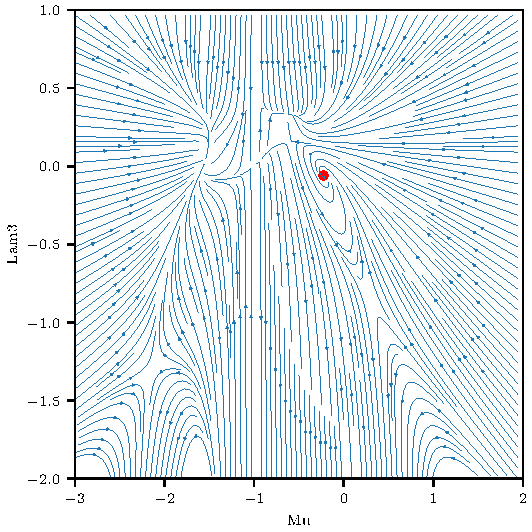
\includegraphics[width=0.48\textwidth]{flow_field_pure2}
	\hfill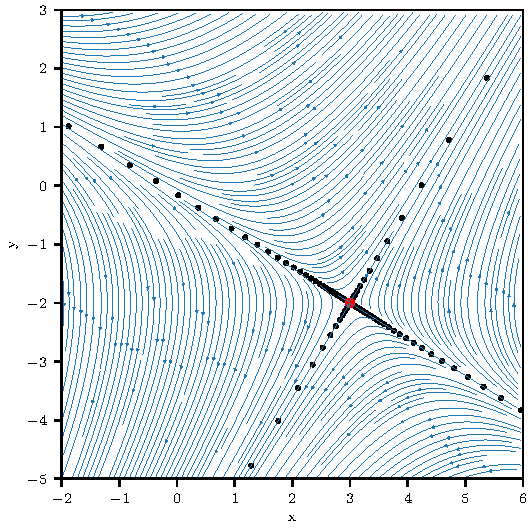
\includegraphics[width=0.48\textwidth]{flow_field1_sep}
	\caption{Flow field of two different sets of ordinary differential equations. Left: The flow of a physical system with five coupling constants, i.e., with a theory space of five dimensions, is shown. In this illustration three couplings are fixed by the three remaining components of the fixed point which corresponds to the red dot. Further fixed points are present for other values for the remaining components. Details on the system and the entire set of flow equations can be found in~\cite{Pawlowski2018}. Right: The saddle point and the extracted separatrices (black dots) are shown for a two-dimensional hyperbolic system.}
	\label{fig:threedimenionsalsystem}
\end{figure*}

Another module provides the possibility to visualise the flow field and the found fixed points in an arbitrary tuple dimensions. In this work, we restrict ourselves to two-dimensional visualisations. Separatrices between given fixed point can also be depicted. We omit a parametrisation of the separatrices in consequence of the complexity of higher-dimensional curved objects. Instead, we detect intersections of the viewed two-dimensional plane and the separatrices on the fly. This is implemented by solving the flow equation for each separatrix for each view by integrating predefined starting points around the saddle points in dependence on the eigenanalysis. The resulting propagation lines span the curved separatrix. If a propagation line is in vicinity of the viewing plane, the intersection is viewed. Examples for resulting flow fields together with detected fixed points and separatrices are shown in Figure~\Cref{fig:threedimenionsalsystem}.

\section{Performance}
\label{sec:performance}

This section presents two performance tests of the developed algorithm with respect to a comparison between the run time on the CPU and on the GPU as well as with respect to the scalability of the algorithm. In particular, we demonstrate a high performance boost for an execution of the fixed point algorithm on the GPU. A comparison to other existing frameworks like Mathematica is subject to future work. Figure~\Cref{fig:performance} shows the correlation between the run time and the dimension for an identity system with a fixed total number of hypercubes to be evaluated. In Figure~\Cref{fig:performance2}, the scalability of the algorithm is investigated artificially with respect to the provided memory of the GPU by a  upper restriction on the number of hypercubes which can be evaluated in parallel.

In both plots, the high performance boost of the algorithm on the GPU becomes visible. This is also due to the efficient data transfer between CPU and GPU of the algorithm itself, as described in~\Cref{sec:algorithms}.

\begin{figure*}
	\centering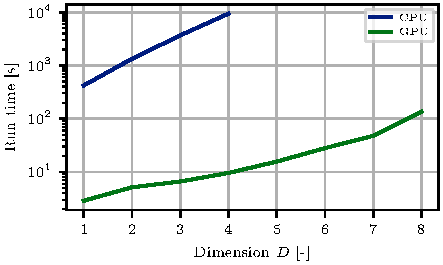
\includegraphics[width=0.7\textwidth]{performance_plot1}
	\caption{The execution time is plotted in dependence of the dimension for an identity system. The total number of hypercubes that need to be evaluated is kept fixed at $10^8$ by choosing a different resolution of the grid within each dimension $D$. The non-linear increase of the curves is a result of the exponentially increasing number of vertices per hypercube of order $\mathcal{O}(2^D)$. Computations on the GPU are significantly faster than on the CPU.}
	\label{fig:performance}
\end{figure*}

\begin{figure*}
	\centering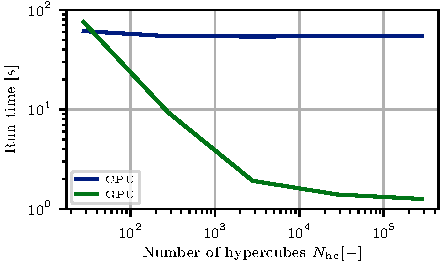
\includegraphics[width=0.7\textwidth]{performance_plot2}
	\caption{The execution time is plotted for a three point system of quantum gravity with a variable total number of hypercubes that can be evaluated in parallel. The theory space has a fixed dimension of three. Details on the considered theory can be found in~\cite{Pawlowski2018}. The plot demonstrates the high performance boost for a reasonable level of parallelisation on the GPU.}
	\label{fig:performance2}
\end{figure*}

\section{Conclusion}
\label{sec:conc}

Within this work, a software framework has been developed which enables a computationally efficient way to find critical points of a set of ordinary differential equations in higher dimensional spaces. A high performance boost is achieved by an implementation of the search algorithm on the GPU. Besides the detection of fixed points, the software offers further features which allow a characterisation of the critical points, a visualisation of the flow field and an evolution in time based on the ODEs for given initial conditions.

The framework might serve as a basis for various investigations of a flow in higher dimensions. This includes both properties of the flow itself and respective methods for a visualisation of vector topology in higher dimensional spaces, in general. Due to the finite scope of this project, implementations of certain features and optimisations is still lacking. For example, an iterative refinement of the resolution of the initial starting points is necessary for a better and more dense detection of intersections between separatrices and other higher dimensional manifolds. With respect to a visualisation of the flow, it is interesting to think about methods to illustrate the sparatrices between different fixed points in lower dimensions. This could be helpful for a better understanding of the interplay of relevant and irrelevant couplings in quantum gravity.

The dimension of the considered theory space is still restricted for the presented algorithm for the detection of fixed points despite the higher computational power by the GPUs. This holds due to the exponentially increasing number of vertices of a hypercube of order $\mathcal{O}(2^D)$. The same holds for the brute force evaluation of hypercubes on a grid. A possible approach to reduce the computation time is to make use of all the information that is present when evaluating a single cube. This includes the position of the hypercube in theory space and the explicitly computed velocities at each vertex. The fixed point search algorithm implemented within this project is based solely on the position and the sign of the flow at the different vertices. A more efficient scan of the theory space should be feasible by methods from the fields of machine learning, statistics and numerical analysis. Estimations about the flow in the vicinity of the considered cube should provide useful information for an exploration of the theory space in a stochastic, iterative manner. Development of such algorithms is subject to future work.

% \addcontentsline{toc}{chapter}{IV Bibliography}
%\nocite{*}
\bibliographystyle{apalike}
%\bibliographystyle{ieeetr}
\bibliography{references}

\end{document}